\subsection{Raspberry Pi}

\begin{frame}{Raspberry Pi}
  \begin{figure}[H]
    \centering
    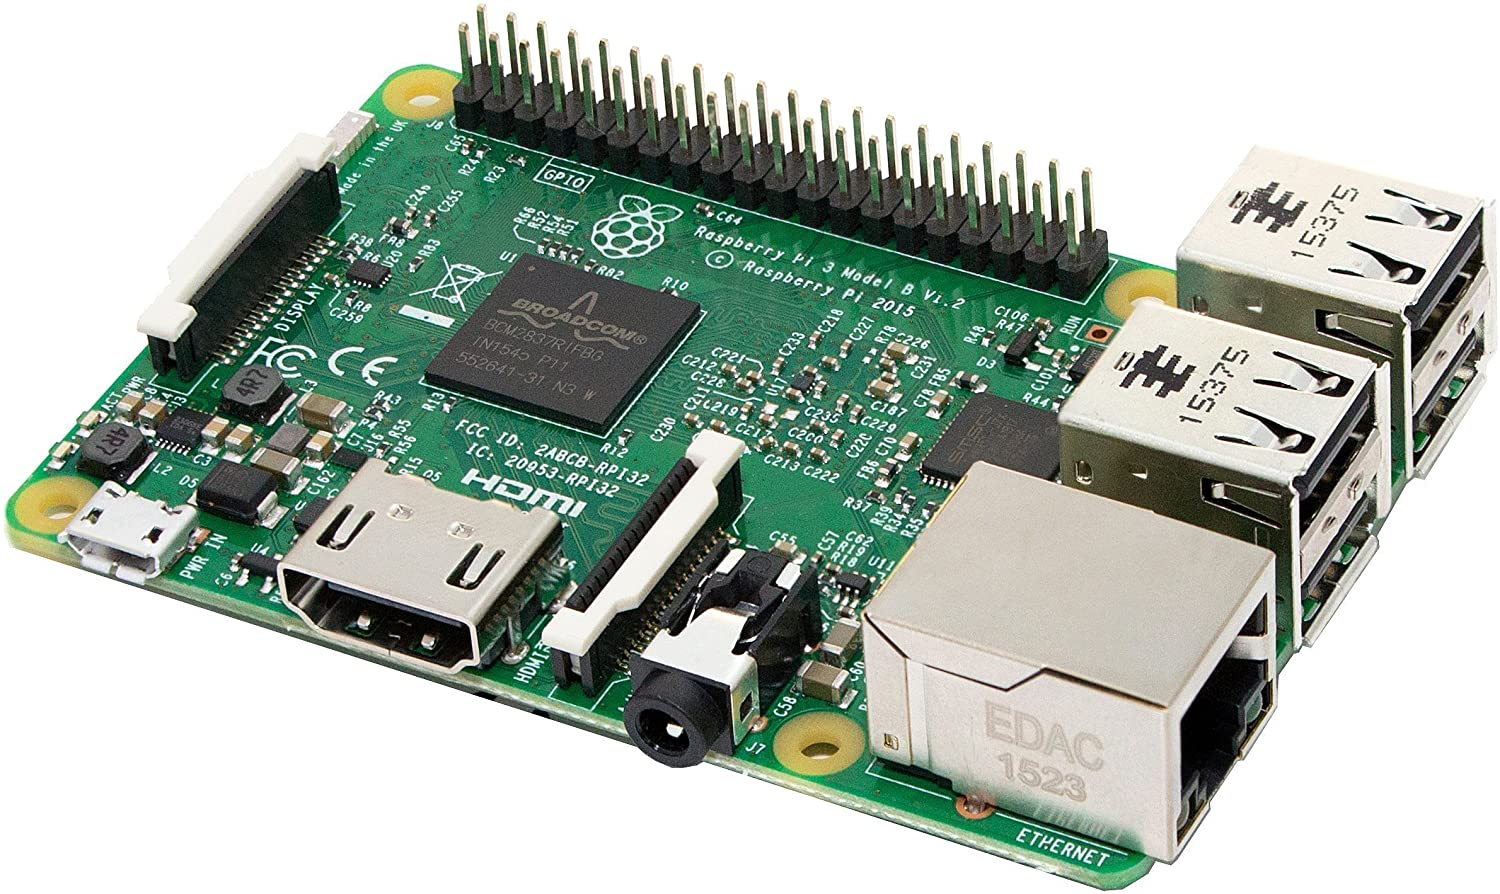
\includegraphics[height=0.75\textheight]{assets/images/rpi__image.jpg}
    \label{img:rpi__image}
  \end{figure}
\end{frame}

\begin{frame}{Raspberry Pi}
  Системные характеристики Raspberry Pi модели 3 B:

  \begin{enumerate}
    \item Микроархитектура --- Cortex-A53 (ARM v8);
    \item Частота центрального процессора --- 1,2 ГГц;
    \item Количество ядер --- 4;
    \item Объём оперативной памяти --- 1 ГБ;
    \item Количество контактов GPIO --- 40;
    \item Количество USB портов --- 4;
    \item Коммуникации --- Ethernet, Wi-Fi, Bluetooth.
  \end{enumerate}
\end{frame}

\subsection{Разработка аппаратной части комплекса}

\begin{frame}{ШИМ}
  ШИМ импульсы управления светодиодами WS2812b

  \begin{figure}[H]
    \centering
    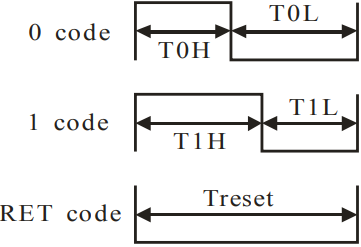
\includegraphics[height=0.65\textheight]{assets/images/PWM__codes.png}
    \label{img:pwm__codes}
  \end{figure}
\end{frame}

% \begin{frame}{ШИМ}
%   Пример ШИМ для кодирования цвета
% 
%   \begin{figure}[H]
%     \centering
%     \includegraphics[width=0.85\textwidth]%  {assets/images/PWM__example.jpg}
%     \label{img:pwm__example}
%   \end{figure}
% \end{frame}

\begin{frame}{GPIO}
  Карта GPIO контактов Raspberry Pi

  \begin{figure}[H]
    \centering
    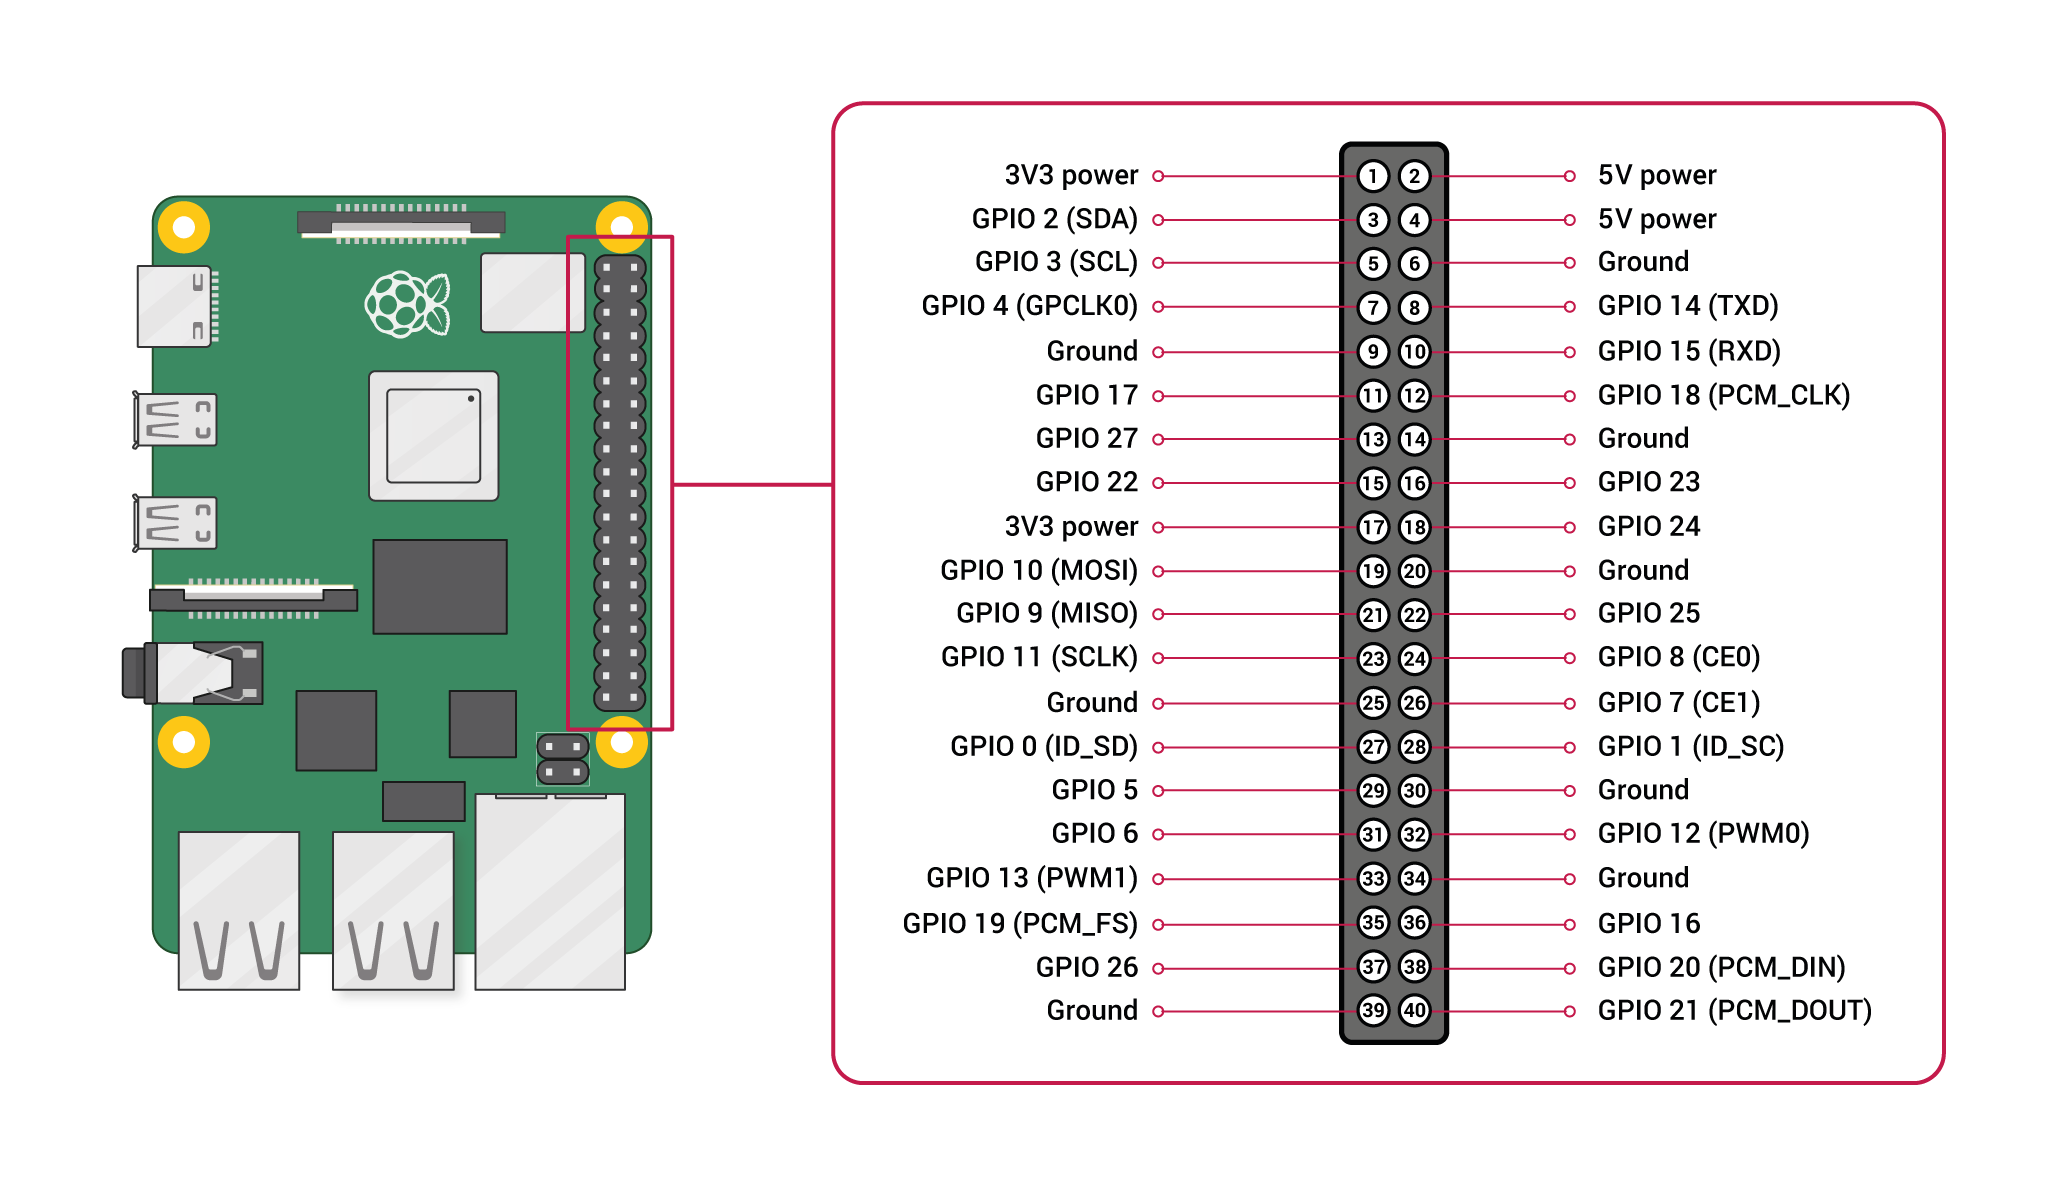
\includegraphics[height=0.75\textheight]{assets/images/GPIO-Pinout-Diagram.png}
  \end{figure}
\end{frame}